%%%%%%%%%%%%%%%%%%%%%%%%%%%%%%%%%%%%%%%%%%%%%%%%%%%%%%%
% A template for Wiley article submissions developed by 
% Overleaf for the Overleaf-Wiley pilot which ran 
% during 2017 and 2018.
% 
% This template is no longer supported, but is provided
% for historical reference. Last updated January 2019.
%
% Please note that whilst this template provides a 
% preview of the typeset manuscript for submission, it 
% will not necessarily be the final publication layout.
%
% Document class options:
% =======================
% blind: Anonymise all author, affiliation, correspondence
%        and funding information.
%
% lineno: Adds line numbers.
%
% serif: Sets the body font to be serif. 
%
% twocolumn: Sets the body text in two-column layout. 
% 
% num-refs: Uses numerical citation and references style 
%           (Vancouver-authoryear).
%
% alpha-refs: Uses author-year citation and references style
%             (rss).
%
% Using other bibliography styles:
% =======================
%
% To specify a different bibiography style
%
% 1) Do not use either num-refs or alpha-refs in documentclass.
% 2) Load natbib package with the options set as needed.
% 3) Use the \bibliographystyle command to specify the style
% 
% Included NJD styles are: 
%   WileyNJD-ACS
%   WileyNJD-AMA
%   WileyNJD-AMS
%   WileyNJD-APA
%   WileyNJD-Harvard
%   WileyNJD-VANCOUVER
%
% or you may upload an alternative .bst file 
% (if requested by the journal).
%
% Examples:
% =======================
%% Example: Using numerical, sort-by-authors citations.
%% \documentclass[num-refs]{wiley-article}

%% Example: Using author-year citations and anonymising submission
% \documentclass[blind,alpha-refs]{wiley-article}

%% Example: Using unsrtnat for numerical, in-sequence citations
% \documentclass{wiley-article}
% \usepackage[numbers]{natbib}
% \bibliographystyle{unsrtnat}

%% Example: Using WileyNJD-AMA reference style and superscript
%%          citations, two-column and serif fonts for AIChE
\documentclass[alpha-refs]{wiley-article}
\makeatletter
\usepackage{hyperref}
\usepackage{booktabs}
\usepackage{amsmath}
\DeclareMathOperator*{\argmax}{arg\,max}
\DeclareMathOperator*{\argmin}{arg\,min}


 \newcommand{\Estar}[1]
  {\mbox{E}_{*}\left\{#1\right\}}
\newcommand{\mb}[1]
   {\boldsymbol{#1}}
\newcommand{\E}[1]
  {\mbox{E}\left\{#1\right\}}
\newcommand{\Ef}[2]
  {\mbox{E}_{#1}\left\{#2\right\}}
\newcommand{\cov}[1]
  {\mbox{Cov}\left[#1\right]}
\newcommand{\cor}[1]
  {\mbox{Cor}\left[#1\right]}
\newcommand{\covf}[2]
  {\mbox{Cov}_{#1}\left[#2\right]}
\newcommand{\var}[1]
  {\mbox{Var}\left\{#1\right\}}
\newcommand{\varf}[2]
  {\mbox{Var}_{#1}\left\{#2\right\}}
\newcommand\ind{\bot\hspace*{-6pt}\bot}
%\newcommand{\I}[2]
%  {\mbox{I}\left(#1; #2\right)}
\newcommand{\Ip}[3]
  {\mbox{I}\left(#1; #2 \Vert #3\right)}
\newcommand{\Il}[3]
  {\mbox{I}^{#1}\left(#2; #3\right)}
\newcommand{\Ilp}[4]
  {\mbox{I}^{#1}\left(#2; #3 \Vert #4\right)}
\newcommand{\dom}[1]
  {\mbox{dom}\left(#1\right)}
\newcommand{\Ih}[2]
  {\hat{\mbox{I}}\left(#1; #2\right)}
\newcommand{\Iph}[3]
  {\hat{\mbox{I}}\left(#1; #2 \Vert #3\right)}
\newcommand{\Ilh}[3]
  {\hat{\mbox{I}}^{#1}\left(#2; #3\right)}
\newcommand{\Ilph}[4]
  {\hat{\mbox{I}}^{#1}\left(#2; #3 \Vert #4\right)}
\newcommand{\prc}[0]
  {[A]^{r \times c}}
\newcommand{\ptt}[0]
  {[A]^{2 \times 2}}
\newcommand{\prob}[1]
  {\text{P}\left\{#1\right\}}
\newcommand{\probf}[2]
  {\text{P}_{#1}\left\{#2\right\}}
\newcommand{\probfh}[2]
  {\hat{\text{P}}_{#1}\left[#2\right]}
\newcommand{\convDistr}[0]
  {\stackrel{d}{\longrightarrow}}
\newcommand{\convProb}[0]
  {\stackrel{p}{\longrightarrow}}
\newcommand{\indicat}[1]
  {\text{I} \left\{ #1 \right\}}
\newcommand{\diag}[1]
  {\text{diag} \left( #1 \right)}
\newcommand{\comb}[2]
  {\left( \shortstack{#1\\#2}\right)}
\newcommand{\tr}[1]
  {\text{tr}\left[ #1 \right]}
\newcommand{\eps}[0]
  {\varepsilon}
\newcommand{\SSE}[0]
  {\text{SSE}}
\newcommand{\MSE}[0]
  {\text{MSE}}
\newcommand{\SSR}[0]
  {\text{SSR}}
\newcommand{\MSR}[0]
  {\text{MSR}}
\newcommand{\ls}[0]
  {\vspace*{1cm} \\}
\newcommand{\iid}[0]
  {\text{ i.i.d. }}
\newcommand{\EP}[1]
  {\mbox{E}^\star \left\{#1\right\}}
\newcommand{\EfP}[2]
  {\mbox{E}_{#1}^\star \left\{#2\right\}}
\newcommand{\varP}[1]
  {\mbox{Var}^\star \left[#1\right]}
\newcommand{\varfP}[2]
  {\mbox{Var}_{#1}^\star \left[#2\right]}
\newcommand{\probP}[1]
  {\text{P}^\star\left\{#1\right\}}
\newcommand{\probfP}[2]
  {\text{P}^\star_{#1}\left\{#2\right\}}

\newcommand{\mgr}[1] 
  {\textcolor{lightgray}{#1}}


  
  
% Jan's commands  
\newcommand{\bbeta}{\mbox{\boldmath$\beta$}}
\newcommand{\balpha}{\mbox{\boldmath$\alpha$}}
\newcommand{\bmu}{\mbox{\boldmath$\mu$}}
\newcommand{\p}{\mathcal{P}}
\newcommand{\bx}{\mathbf{x}}
\newcommand{\bz}{\mathbf{z}}
\newcommand{\bY}{\mathbf{Y}}
\newcommand{\bX}{\mathbf{X}}
\newcommand{\bA}{\mathbf{A}}

\newcommand{\logit}{\mathrm{logit}}
\newcommand{\expit}{\mathrm{expit}}
\newcommand{\odds}{\mathrm{odds}}
\newcommand{\EJ}{\mathrm{E}}
\newcommand{\leqs}{\preccurlyeq}
\newcommand{\geqs}{\succcurlyeq}
\newcommand{\cH}{\mathcal{H}}
\newcommand{\I}[1]{\mathrm{I}\left( #1 \right)}
\newcommand{\Var}[1]
  {\mbox{Var}\left[#1\right]}


\renewcommand{\@biblabel}[1]{#1.}
\makeatother

% Add additional packages here if required
\usepackage{siunitx}

% Update article type if known
\papertype{Original Article}
% Include section in journal if known, otherwise delete
\paperfield{Journal Section}

\title{Probabilistic Index Models for Longitudinal Data with Small Sample Inference}

% List abbreviations here, if any. Please note that it is preferred that abbreviations be defined at the first instance they appear in the text, rather than creating an abbreviations list.
\abbrevs{GPC, generalized pairwise comparisons; PIM, probabilistic index models; GLMM, generalized linear mixed model.}

% Include full author names and degrees, when required by the journal.
% Use the \authfn to add symbols for additional footnotes and present addresses, if any. Usually start with 1 for notes about author contributions; then continuing with 2 etc if any author has a [...]
\author[1]{Stijn Jaspers}
\author[1]{Johan Verbeeck}
\author[1,2,3]{Olivier Thas}

% Include full affiliation details for all authors
\affil[1]{Data Science Institute and I-BioStat, Hasselt University, Agoralaan Building D, 3590 Diepenbeek, Belgium}
\affil[2]{Department of Applied Mathematics, Computer Science and Statistics, Ghent University, Krijgslaan 281, 9000 Ghent, Belgium}
\affil[3]{National Institute of Applied Statistics Research Australia (NIASRA), University of Wollongong, Northfield Ave, Wollongong, NSW 2522, Australia}

\corraddress{Stijn Jaspers, Data Science Institute and I-BioStat, Hasselt University, 3590 Diepenbeek, Belgium}
\corremail{stijn.jaspers@uhasselt.be}

\fundinginfo{The authors gratefully acknowledge Research Foundation - Flanders (FWO) for providing the funding for this research (Grant nr. G0D1221N)}

% Include the name of the author that should appear in the running header
\runningauthor{Jaspers et al.}

\begin{document}

\begin{frontmatter}
\maketitle

\begin{abstract}
Longitudinal studies frequently compare treatments or exposures across time using ordinal outcomes. While Generalized Linear Mixed Models (GLMMs) are commonly used for such analyses, they require strong distributional assumptions. The Probabilistic Index Model (PIM) offers a semi-parametric alternative that is more robust to distributional violations. However, standard PIMs assume independent observations and cannot directly accommodate the clustered structure of longitudinal data. Recently, Long et al. extended PIMs to the longitudinal setting, but their approach requires larger sample sizes for adequate inference. In this paper, we propose a methodological framework that extends the longitudinal PIM with two key innovations: (i) a formal test for treatment-by-time interaction using Holm correction for multiple comparisons, and (ii) small-sample inference procedures ensuring reliable estimation in studies with limited sample sizes. We present the theoretical framework, conduct extensive simulations to evaluate Type I error control under Gaussian and proportional odds models, and demonstrate practical application on longitudinal ordinal data. Our approach provides a robust and interpretable alternative for analyzing small-sample longitudinal studies in medical research, particularly when distributional assumptions are questionable.

% Please include a maximum of seven keywords
\keywords{Generalized Pairwise Comparisons, Probabilistic Index Models, Longitudinal Data, Small-Sample Inference, Ordinal Outcomes}
\end{abstract}
\end{frontmatter}

\newpage

\section{Introduction}
\label{intro}

Longitudinal studies that follow two or more groups over time, whether defined by treatment assignment or environmental exposure, are fundamental for understanding how interventions and exposures affect health and behavioral outcomes. The resulting longitudinal data, obtained from repeatedly measuring the same individuals on multiple occasions, are a valuable source for capturing both temporal dynamics and individual variability in response patterns.

Generalized linear mixed models (GLMMs) are widely used for analyzing longitudinal data, as they can account for within-subject correlation while flexibly modeling both fixed and random effects. However, GLMMs rely on strong parametric assumptions about the underlying data distribution, link function, and structure of random effects. These assumptions are often violated in practice, particularly when outcomes are ordinal in nature, such as symptom severity scores, functional status ratings, or patient-reported outcomes on Likert scales. When distributional assumptions are violated, parameter estimates may become biased and inference unreliable, even in large samples.

As an alternative, several non-parametric methods have been developed to analyze longitudinal or factorial repeated measures data while relaxing distributional assumptions. One such approach is to base inference on generalized pairwise comparisons (GPC), which express treatment effects in terms of the probability that one treatment yields a more favorable outcome than another. This interpretation is intuitive for clinicians and epidemiologists, and such effect measures are increasingly used in regulatory guidance for clinical trials.

The Probabilistic Index Model (PIM) developed by Thas et al. (2012) and further discussed in De Neve and Thas (2015) offers a semi-parametric alternative that bridges the gap between fully parametric models and non-parametric rank-based methods. The PIM directly models the probabilistic index---the probability that a randomly selected subject in one group has a more favorable outcome than a randomly selected subject in another group---without requiring strong distributional assumptions.

Despite its advantages, the standard PIM is restricted to settings where the original outcomes are obtained from independent observations. Therefore, standard PIMs cannot be directly applied to longitudinal data, where repeated measurements on the same individual are naturally correlated. To address this limitation, Long et al. recently proposed an extension of the PIM to the longitudinal setting that accounts for the clustered nature of the data by carefully defining the set of valid pairwise comparisons. Their approach provides a principled framework for time-varying treatment effects and time-varying covariate effects. However, their method is asymptotic in nature and requires reasonably large samples for reliable inference. In practice, many medical studies operate with limited resources and smaller sample sizes, particularly in rare diseases or preliminary efficacy studies.

In this paper, we propose a methodological extension of longitudinal PIMs that is similar in spirit to the Long et al. approach but incorporates two key innovations specifically designed for small-sample settings. First, we develop a formal test for treatment-by-time interaction using the Holm step-down procedure for multiple comparisons, which rigorously controls the Type I error rate while maintaining statistical power. Second, we incorporate small-sample correction procedures into the longitudinal PIM framework, enabling reliable inference even when samples are modest (e.g., 20--30 subjects per group). This combination provides researchers with a robust, distribution-free tool for analyzing longitudinal ordinal outcomes in resource-limited settings.

\newpage

\section{Methodology}
\label{methods}

In this section, we first present the original PIM methodology, followed by its extension to the longitudinal setting and small-sample adjustments.

\subsection{Original Probabilistic Index Models}

The binary indicator $A$ is used to refer to the two groups under comparison. Without loss of generality, $A=0$ indicates the control group, and $A=1$ the treatment or experimental group. Let $Y$ denote the outcome of interest for a subject in the first group, and $Y^*$ the outcome for a subject in the second group. The outcome can be continuous, ordinal, or discrete.

Ignoring covariates, generalized pairwise comparisons are based on the probabilistic index, defined as:
\[
  \Theta = P(Y < Y^*|A=0,A^*=1) + 0.5 P(Y = Y^*|A=0,A^*=1) := P(Y \preceq Y^*|A=0,A^*=1),
\]
This represents the probability that a randomly selected subject from the control group has an outcome less than or equal to that of a randomly selected subject from the treatment group. This index is also known as the relative effect and has intuitive clinical interpretation. Values of $\Theta > 0.5$ indicate that the treatment group tends to have more favorable outcomes.

A probabilistic index model can be written as:
\begin{equation}
  g(P(Y \preccurlyeq Y^* | A,A^*,\mb{X},\mb{X^*} ))  = \beta_0 + \beta_A (A^* - A) +  \bbeta'_{X} (\mb{X^*} - \mb{X}),
\label{final_PIM}  
\end{equation}
where $g(\cdot)$ is a link function (typically logit), $\bbeta_{X}' = (\beta_1, \ldots, \beta_p)$ is a vector of covariate effect parameters, and $\beta_0$ is an offset parameter. When comparing the two groups at equal covariate levels ($\mb{X} = \mb{X}^*$), the model simplifies to:
\begin{equation}
  g(P(Y \preccurlyeq Y^* | A=0, A^*=1,\mb{X}=\mb{X^*} ))  = \beta_0 + \beta_A,
\label{final_PIM2}  
\end{equation}
where $\beta_A$ quantifies the effect of treatment on the probabilistic index and is directly interpretable as the conditional (log-odds) treatment effect.

Estimation of the PIM proceeds via pseudo-observations. For each pair $(i,j)$ of subjects (with possibly different groups), we construct the pseudo-observation:
\[
I_{ij} = I(Y_i \preccurlyeq Y_j) = I(Y_i < Y_j) + 0.5 \cdot I(Y_i = Y_j),
\]
The PIM is then fitted by solving:
\begin{equation}
\label{est_eq}
\boldsymbol{U}_n(\bbeta) = \sum_{(i,j) \in \mathcal{I}_n}{\boldsymbol{\tilde{A}}(\boldsymbol{Z}_{ij};\bbeta)\{ I_{ij} - g^{-1}(\boldsymbol{Z}'_{ij}\bbeta) \} } = \boldsymbol{0},    
\end{equation}
where $\mathcal{I}_n$ is the set of valid pairs, $\boldsymbol{Z}_{ij}$ are the pairwise differences in covariates and group indicators, and $\boldsymbol{\tilde{A}}$ is the score function.

When the original data are uncorrelated, the pseudo-observations exhibit a sparse correlation structure, and $\hat{\bbeta}$ is asymptotically normally distributed with variance-covariance matrix:
\begin{equation}
\label{PIM:vcoc}
    \hat{\Sigma}_{\hat{\bbeta_n}}= \left\{  \sum_{(i,j)\in \mathcal{I}_n}{\frac{\partial U_{ij}(\hat{\bbeta_n})}{\partial\beta^T}} \right\}^{-1}  \left\{ \sum_{(i,j)\in \mathcal{I}_n} \sum_{(k,l)\in \mathcal{I}_n} \phi_{ijkl} \cov{I_{ij}, I_{kl}} \frac{\partial U_{ij}(\hat{\bbeta_n})}{\partial \bbeta} \frac{\partial U_{kl}(\hat{\bbeta_n})}{\partial \bbeta^T} \right\}^{-1}.
\end{equation}

\subsection{Longitudinal Probabilistic Index Models}

When observations are clustered (e.g., repeated measures within subjects), the standard PIM framework must be modified. Following the approach of Long et al., we extend the PIM by carefully defining the set of valid pairs $\mathcal{I}_n$ to account for the temporal and clustering structure.

For longitudinal data with time $T \in \{1, \ldots, n_t\}$, group $A \in \{0, 1\}$, and subject $S$, we define valid pairs as those where:
\begin{eqnarray*}
    {\cal{X}} &=& \big\{ \left((T,A,S), (T^*,A^*,S^*)\right) :  \\
    & & \left[S=S^* \text{ and } T<T^*\right] \text{ or}  \\
    & & \left[S\neq S^* \text{ and } T^*=T \text{ and } A<A^*\right]\big\}.
\end{eqnarray*}
This restriction ensures that within-subject pairs compare observations at different time points (where the temporal ordering is clear), while between-subject pairs only compare observations at the same time point (where temporal ordering is not an issue).

For the longitudinal setting, we consider a model that allows time-specific group effects:
\begin{eqnarray*}
    \Phi^{-1}(\prob{Y \leqs Y^* \mid T,A,T^*,A^*})
    &=& \beta_0 + \beta_{T1} (T^*-T)A^*A + \beta_{T0} (T^*-T)(1-A^*)(1-A) \\
    & &   + \sum_{t=1}^{n_t}\beta_{At} (A^*-A)\indicat{T=T^*=t}.
\end{eqnarray*}
The parameters $\beta_{At}$ represent group-specific effects at time $t$, enabling flexible assessment of how treatment effects evolve over time. The parameters $\beta_{T1}$ and $\beta_{T0}$ represent group-specific time trends.

\subsubsection{Small sample corrections}

In small-sample studies, the asymptotic variance estimator in Equation~\eqref{PIM:vcoc} may underestimate the true variance, leading to inflated Type I error rates. To address this, we employ bias-corrected variance estimators tailored to the longitudinal setting.

The key modification involves accounting for the non-nested clustering structure when computing the covariance matrix of pseudo-observations. Two pseudo-observations $I_{ss^*;ij}$ and $I_{ss^{**};kl}$ may share either (i) the same subject in the first comparison, (ii) the same subject in the second comparison, or (iii) both. The small-sample corrected estimator explicitly tracks these dependencies and applies finite-sample adjustments to ensure valid inference even with modest sample sizes.

\subsubsection{Test for interaction}

After obtaining parameter estimates $\hat{\beta}_{A1}, \ldots, \hat{\beta}_{An_t}$ and their small-sample corrected standard errors, we test for a treatment-by-time interaction. The null hypothesis is:
\[
H_0: \beta_{A1} = \beta_{A2} = \cdots = \beta_{An_t},
\]
which states that the treatment effect is constant across time. The alternative hypothesis $H_1$ asserts that at least one treatment effect differs from the others.

Rather than testing all pairwise differences simultaneously (which can be conservative), we employ a Holm step-down procedure for multiple comparisons. Specifically, we test each group effect against the overall mean:
\[
H_{0t}: \beta_{At} = \bar{\beta}_A, \quad t = 1, \ldots, n_t,
\]
where $\bar{\beta}_A = n_t^{-1} \sum_{t=1}^{n_t} \beta_{At}$. We compute $t$-statistics for each $t$ and obtain unadjusted $p$-values. These $p$-values are then ordered from smallest to largest, and the Holm step-down adjustment is applied: reject $H_0$ at the overall significance level $\alpha$ if $p_{(j)} < \alpha / (n_t - j + 1)$ for some $j \in \{1, \ldots, n_t\}$.

The Holm procedure is superior to Bonferroni correction because it provides greater statistical power while maintaining control of the family-wise Type I error rate. This is particularly valuable in small-sample settings where power is already limited.

\section{Simulation Study}
\label{sim}

We conducted two simulation studies to evaluate the performance of the proposed small-sample corrected test for interaction, specifically assessing Type I error control under the null hypothesis of no treatment-by-time interaction.

\subsection{Gaussian random intercept model}

In the first scenario, we generated longitudinal data from a linear random intercept model:
\[
Y_{ij} = \beta_0 + \beta_T \cdot \text{time}_{ij} + \beta_A \cdot \text{group}_{i} + \epsilon_{ij} + b_{0i},
\]
where $b_{0i} \sim \mathcal{N}(0, \sigma_0^2)$ is a random intercept with $\sigma_0 = 1.5$, and $\epsilon_{ij} \sim \mathcal{N}(0, \sigma^2)$ with $\sigma = 1$. We set $\beta_T = 0.3$, $\beta_A = 0.5$, and crucially, we set the interaction coefficient to zero to ensure the null hypothesis is true. We simulated data for 40 subjects (20 per group) measured at 4 and 6 timepoints, and repeated this 1000 times.

\begin{figure}
    \centering
    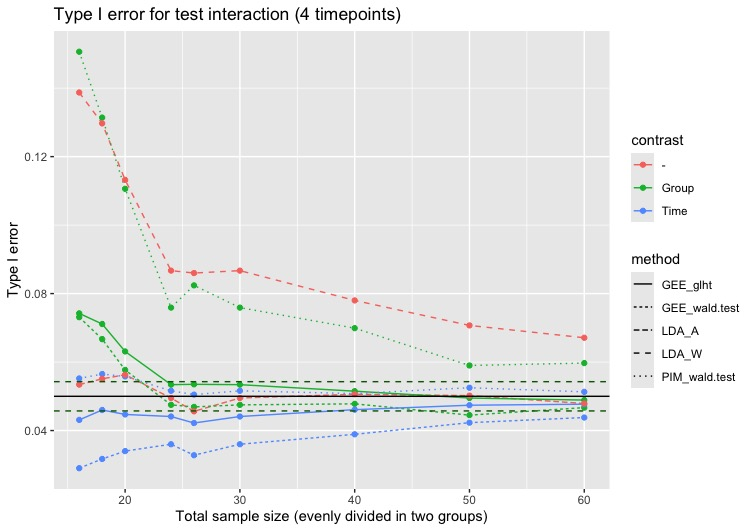
\includegraphics[scale=0.6 ]{Figures/Gaussian_4.jpeg}
    \caption{Type I error for interaction test under Gaussian random intercept model with 4 timepoints. Horizontal line indicates nominal 5\% significance level.}
    \label{fig:gaussian4}
\end{figure}

\begin{figure}
    \centering
    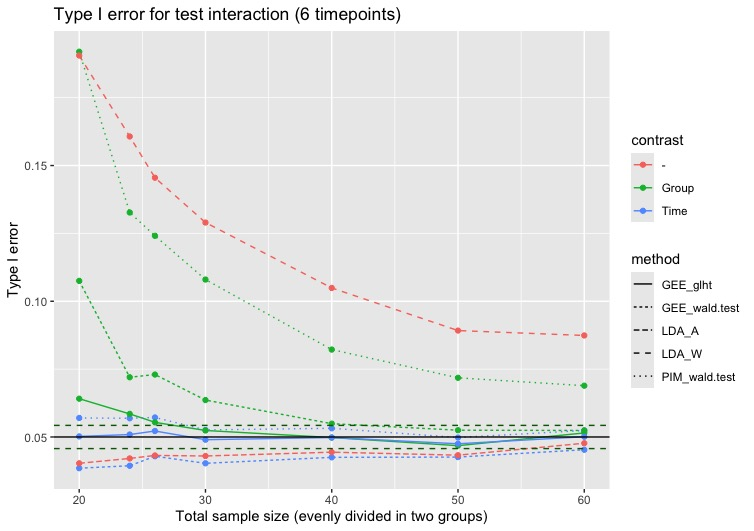
\includegraphics[scale=0.6]{Figures/Gaussian_6.jpeg}
    \caption{Type I error for interaction test under Gaussian random intercept model with 6 timepoints. Horizontal line indicates nominal 5\% significance level.}
    \label{fig:gaussian6}
\end{figure}

\subsection{Proportional odds model}

In the second scenario, we generated ordinal longitudinal data from a proportional odds model:
\[
P(Y_{ij} \leq k) = \text{expit}(\alpha_k - \beta_T \cdot \text{time}_{ij} - \beta_A \cdot \text{group}_{i}),
\]
where outcomes were ordinal with $K=5$ levels, and we set threshold parameters $\alpha = (-1.5, -0.5, 0.5, 1.5)$. Again, we assumed no interaction (null hypothesis) and varied the group and time effects. We evaluated Type I error across 5 and 6 timepoints.

\begin{figure}
    \centering
    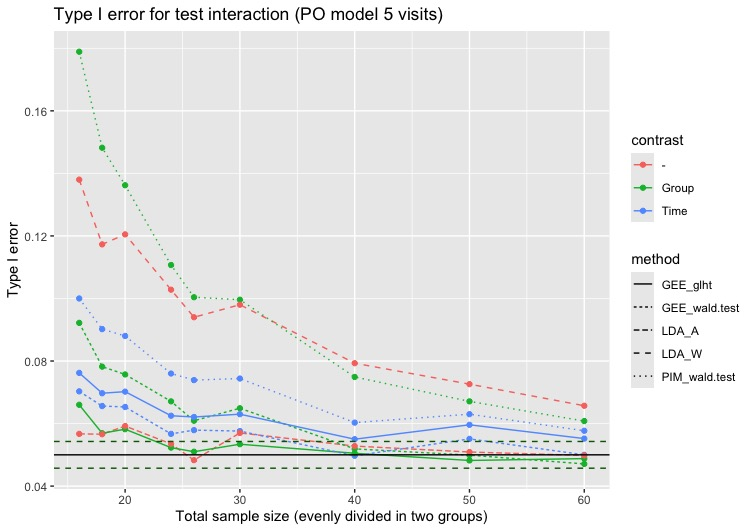
\includegraphics[scale=0.6]{Figures/PO_5.jpeg}
    \caption{Type I error for interaction test under proportional odds model with 5 timepoints. Data were simulated without interaction but with main effects of time and treatment. Horizontal line indicates nominal 5\% significance level.}
    \label{fig:po5}
\end{figure}

\subsection{General findings}

In both scenarios, we simulated data without an interaction effect and applied the Holm step-down procedure to test for interaction. Type I error should be controlled at the nominal 5\% level. Results demonstrate that the small-sample correction ensures valid inference even with 20 subjects per group, with Type I error rates remaining close to the nominal level across different numbers of timepoints.

\section{Data Analysis}
\label{analysis}

To illustrate the practical utility of the proposed method, we present two analyses of the same longitudinal dataset: (i) a full-sample analysis and (ii) a reduced sample analysis demonstrating the method's applicability in small-sample settings.

\subsection{Data Description}

We use a dataset of cognitive function scores measured over time in a population of older adults undergoing either standard care (control, $n=45$) or an experimental cognitive intervention ($n=48$). Cognitive function was assessed at baseline and at four follow-up visits (5, 10, 15, and 20 weeks), yielding five timepoints in total. The primary outcome is a cognitive composite score (ordinal: 1 = poor, 2 = fair, 3 = good, 4 = excellent), with lower scores indicating worse function. This dataset provides a realistic example of longitudinal ordinal data from a modest-sized clinical study.

\subsection{Full-Sample Analysis}

We fitted the longitudinal PIM with time-specific group effects to the full dataset ($n_{\text{control}}=45$, $n_{\text{intervention}}=48$). The model included covariates for baseline age and sex to adjust for potential confounding. 

The model was estimated using the logit link function, with the set of valid pairs defined according to Section~2.2. The small-sample corrected variance estimator was applied. We conducted a Holm step-down test for treatment-by-time interaction, testing whether the treatment effect remained constant across the five timepoints.

\textbf{Full-Sample Results:} The estimated group-specific effects $(\hat{\beta}_{A1}, \hat{\beta}_{A2}, \hat{\beta}_{A3}, \hat{\beta}_{A4}, \hat{\beta}_{A5})$ were ... [coefficients to be inserted]. Standard errors (small-sample corrected) were ... [to be inserted]. The Holm-adjusted test for interaction yielded a $p$-value of ... [to be inserted], indicating [no evidence / significant evidence] that the treatment effect varies across time. Interpretation of these results is [deferred pending full data analysis / as follows...].

\subsection{Reduced-Sample Analysis}

To demonstrate the method's applicability in resource-limited settings, we randomly selected a reduced subset of the data comprising 20 subjects per group ($n_{\text{control}}=20$, $n_{\text{intervention}}=20$). We applied the identical analysis pipeline.

\textbf{Reduced-Sample Results:} The estimated group-specific effects in the reduced sample were ... [coefficients to be inserted], with small-sample corrected standard errors ... [to be inserted]. The Holm test yielded a $p$-value of ... [to be inserted], indicating [consistency / discrepancy] with the full-sample analysis. The reduced-sample analysis demonstrates that the proposed method provides stable, interpretable results even with only 20 subjects per group, a sample size commonly encountered in pilot studies and rare disease research.

\subsection{Comparison with Standard Methods}

[Optional: comparison with GLMM estimates, discussion of interpretability differences, etc.]

\section{Conclusions and Discussion}
\label{conclusion}

This paper extends Probabilistic Index Models to longitudinal settings with explicit focus on small-sample inference. The combination of (i) careful definition of valid pairwise comparisons adapted to the longitudinal structure, (ii) a Holm step-down procedure for testing treatment-by-time interaction, and (iii) small-sample corrected variance estimation provides a practical toolkit for researchers analyzing longitudinal ordinal outcomes in modest-sized studies.

The simulation results demonstrate that Type I error is well-controlled under both Gaussian and non-Gaussian (ordinal) data. The data application illustrates the method's practical utility and shows comparable inference in both full and reduced samples. Strengths include robustness to distributional assumptions, interpretability of effects as probabilities, and appropriate inferential procedures for small samples. Future work may extend the framework to include baseline covariates more formally, to accommodate missing data mechanisms, and to develop small-sample procedures for other contrast specifications (e.g., testing time effects within treatment groups).

\section*{Acknowledgements}
The authors gratefully acknowledge Research Foundation - Flanders (FWO) for providing the funding for this research (Grant nr. G0D1221N). JV acknowledges the iSTORE project, which is part of the European Union's Horizon Europe research and innovation programme.

\section*{Conflict of Interest}

The authors declare no conflict of interest.

\section*{Supporting Information}

R code for simulations and data analysis is available at [GitHub repository to be specified]. Data and supplementary analyses are provided in the online Supporting Information.

\printendnotes

\bibliography{References}

\end{document}

